\section{Modelization of a DC-DC converter}
In the system we want to simulate, as in many real-life systems, is present a DC-DC converter, which will have its non-idealities too, resulting in energy losses.

This means, while in an ideal DC-DC converter the input and output power will be equal ($P_{in}=P_{out}$), in a real one the output power will be scaled by a factor $\eta$, and thus it will be $\eta P_{in}=P_{out}$. $\eta$ will be called \emph{efficiency} of the DC-DC converter. in order to simulate the blocks into SimuLink, we wanted to find a good expression approximating the power loss due to the non-unary efficiency ($P_{loss}$). The chosen analytical expression to fit on the $P_{loss}$ data has been a quadratic one:
$$
P_{loss}=c_1I_{out}^2+c_2I_{out}+c_3
$$

As in the previous part, the first work has consisted in extrapolating data from a graph present into the datasheet of the converter (\emph{LTC3789}), in order to obtain a current-efficiency curve. It has been important to notice that the data were in logarithmic scale on the X axis, and so have had to be interpolated as exponents and transformed into linear values post-audit.

After extracting data from the graph and linearly interpolating it, in order to fit the analytical onto the $P_{loss}$ data it has been needed to use the relationship (which is valid by definition of $\eta$) between $\eta$ and $P_{loss}$:
\begin{gather*}
\eta=\frac{P_{out}}{P_{in}} \\
\Downarrow \\
\eta=\frac{P_{out}}{P_{out}+P_{loss}}
\end{gather*}

Instead of reverting this equation and doing a two-step process to fit the curve, again the \emph{fmins} has been used to evaluate fitting between the available $\eta$ data and the new $P_{loss}$ data. The handle passed to \emph{fmins} calls a function which evaluates the expected $\eta$ vector starting from a sample $P_{loss}$ vector, compares it with the actual $\eta$ vector and returns the squared difference (i.e. the error) between the two. Minimizing this cost function is equivalent to fitting the $P_{loss}$ curve to the desired one.

Again, the result has been satisfactory enough.

\begin{center}
\begin{tabular}{|c| c|}

    \hline
    Parameter name & Parameter value \\
    \hline
    $c_{1}$ & 0.0309 \\
    $c_{2}$ & 0.1166 \\
    $c_{3}$ & 0.4535 \\
    \hline
\end{tabular}

\begin{figure}[h]
  \centering
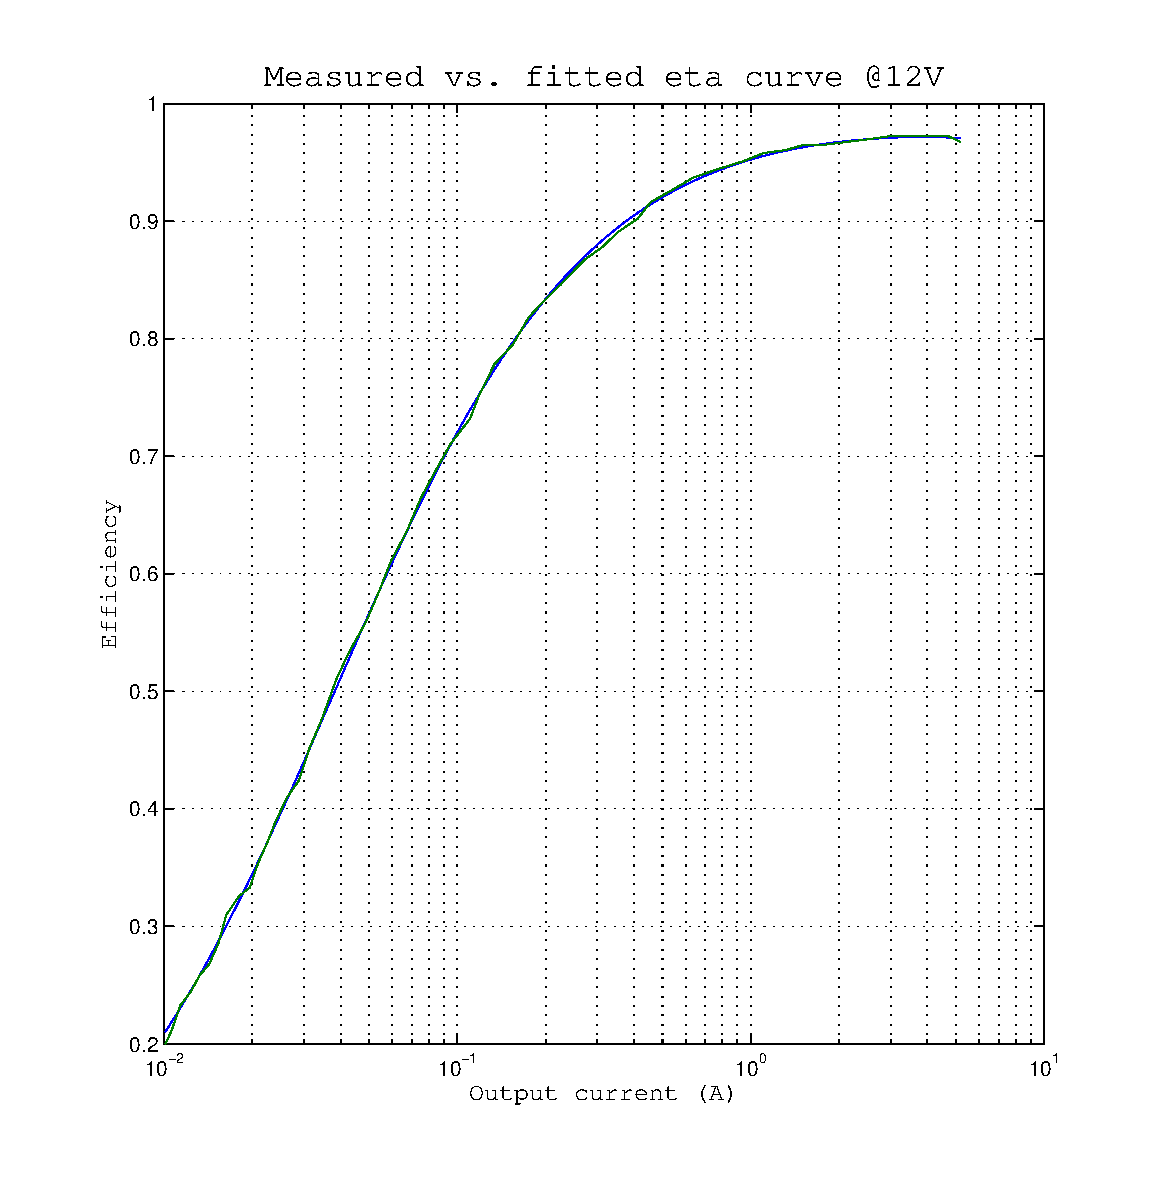
\includegraphics[width=2.5in]{fitted_eta}
\caption{Current-Efficiency curve as computed after fitting $P_{loss}$}
\end{figure}
\begin{figure}[h]
  \centering
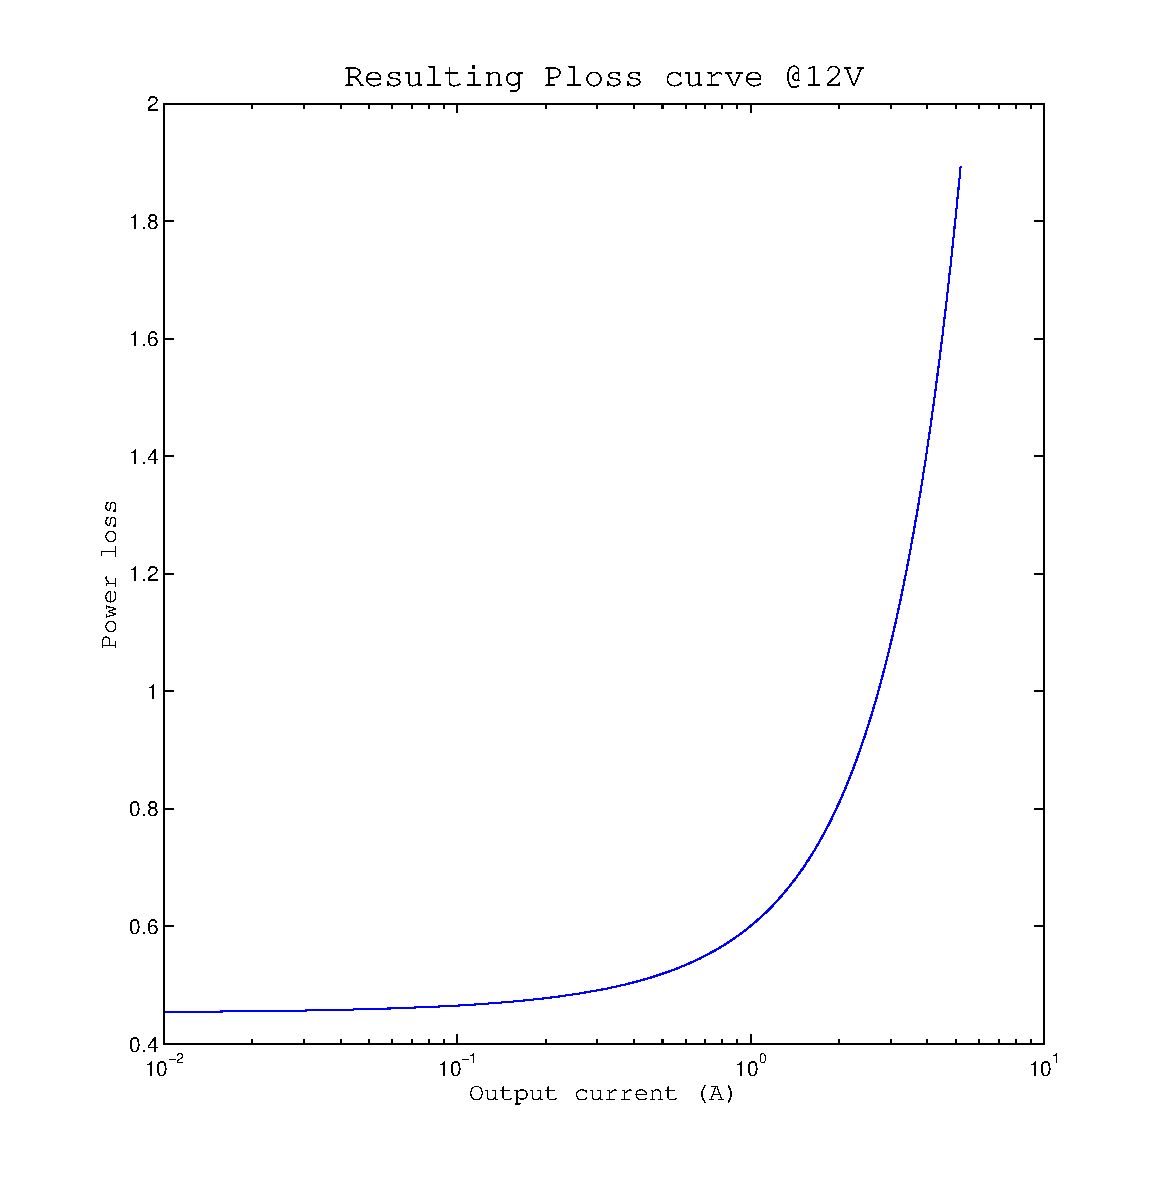
\includegraphics[width=2.5in]{ploss}
\caption{Obtained Current-Power loss curve for the converter}
\end{figure}

\end{center}
